\documentclass[12pt,a4]{article}\usepackage[]{graphicx}\usepackage[]{xcolor}
% maxwidth is the original width if it is less than linewidth
% otherwise use linewidth (to make sure the graphics do not exceed the margin)
\makeatletter
\def\maxwidth{ %
  \ifdim\Gin@nat@width>\linewidth
    \linewidth
  \else
    \Gin@nat@width
  \fi
}
\makeatother

\definecolor{fgcolor}{rgb}{0.345, 0.345, 0.345}
\newcommand{\hlnum}[1]{\textcolor[rgb]{0.686,0.059,0.569}{#1}}%
\newcommand{\hlstr}[1]{\textcolor[rgb]{0.192,0.494,0.8}{#1}}%
\newcommand{\hlcom}[1]{\textcolor[rgb]{0.678,0.584,0.686}{\textit{#1}}}%
\newcommand{\hlopt}[1]{\textcolor[rgb]{0,0,0}{#1}}%
\newcommand{\hlstd}[1]{\textcolor[rgb]{0.345,0.345,0.345}{#1}}%
\newcommand{\hlkwa}[1]{\textcolor[rgb]{0.161,0.373,0.58}{\textbf{#1}}}%
\newcommand{\hlkwb}[1]{\textcolor[rgb]{0.69,0.353,0.396}{#1}}%
\newcommand{\hlkwc}[1]{\textcolor[rgb]{0.333,0.667,0.333}{#1}}%
\newcommand{\hlkwd}[1]{\textcolor[rgb]{0.737,0.353,0.396}{\textbf{#1}}}%
\let\hlipl\hlkwb

\usepackage{framed}
\makeatletter
\newenvironment{kframe}{%
 \def\at@end@of@kframe{}%
 \ifinner\ifhmode%
  \def\at@end@of@kframe{\end{minipage}}%
  \begin{minipage}{\columnwidth}%
 \fi\fi%
 \def\FrameCommand##1{\hskip\@totalleftmargin \hskip-\fboxsep
 \colorbox{shadecolor}{##1}\hskip-\fboxsep
     % There is no \\@totalrightmargin, so:
     \hskip-\linewidth \hskip-\@totalleftmargin \hskip\columnwidth}%
 \MakeFramed {\advance\hsize-\width
   \@totalleftmargin\z@ \linewidth\hsize
   \@setminipage}}%
 {\par\unskip\endMakeFramed%
 \at@end@of@kframe}
\makeatother

\definecolor{shadecolor}{rgb}{.97, .97, .97}
\definecolor{messagecolor}{rgb}{0, 0, 0}
\definecolor{warningcolor}{rgb}{1, 0, 1}
\definecolor{errorcolor}{rgb}{1, 0, 0}
\newenvironment{knitrout}{}{} % an empty environment to be redefined in TeX

\usepackage{alltt}

% ---- Metadata ---- %

\title{Honesty by Convenience: Corruption Tolerance in Ecuador}
\author{Daniel Sánchez}
\date{June 2022}

% ---- Load Packages ---- %

% Math

\usepackage{savesym} % Need to "save" the command that is already defined \varTheta

\usepackage{amsmath}
  \savesymbol{varTheta} 

% Fonts

% To set the TNR font for both text and equations:

\usepackage{mathspec}
  \setallmainfonts(Digits,Greek,Latin){Times New Roman}
\restoresymbol{MTP}{varTheta}

% Formatting

\usepackage{setspace}
  \doublespacing

\usepackage[margin = 1in]{geometry}

\usepackage{lscape}

% Setting the size of the section titles

\usepackage{titlesec}

\titleformat*{\section}{\normalsize\bfseries}

% Citation & Bibliographies

\usepackage[backend = biber, style = apa, citestyle = apa]{biblatex}
  \addbibresource{refs.bib}
  
% For tables:

 % For the modelsummary tables:
\usepackage{siunitx}
\usepackage{booktabs} 
  \newcolumntype{d}{S[input-symbols = ()]}
\usepackage{multirow}
\usepackage[flushleft]{threeparttable}

% For figure and table captions

\usepackage{caption}
  \captionsetup{labelfont = bf} % All in bold  
  
% Other packages

\usepackage{csquotes} % For quotation marks

\usepackage{epigraph} % For epigraph
  \setlength\epigraphwidth{9cm}
  \setlength\epigraphrule{1pt}

\usepackage{float} % For the H float option- only used in emergencies (lol)

\usepackage{textcomp} % For the registered trademark symbol.

% Always load these packages at the end of the preamble:

\usepackage{hyperref}

% ---- R Stuff to be used in the whole document ----

% Here I will execute or source R code through chunks that I need to use throughout the whole document.

% General settings



% Load the data by sourcing the data manipulation script. Note that survey design objects are indeed created in this script.


\IfFileExists{upquote.sty}{\usepackage{upquote}}{}
\begin{document}

% ---- Sections ---- %

% Abstract Child Document


% Abstract .Rnw File


\begin{center}
\textbf{
Honesty by Convenience: Corruption Tolerance in Ecuador\\
Daniel Sánchez}
\end{center}

\textit{
Attitudes towards corruption may be a strong determinant of its incidence. Using survey
data from the AmericasBarometer (AB), binary-outcome empirical models are estimated to discover
the key determinants of an increase in corruption tolerance in Ecuador between 2014 and
2016. It is found that two key variables may have influenced this increase. People who approved
of the President’s job performance initially justified bribes less, but by 2016 supporters justified corruption more. Also, those who identified closer to the political right justified corruption more in 2016. The jump is explained through these variables as the percentage of people who approved of the President decreased and the percentage of people identifying with the right increased. It is also found that the people who were either employed or outside the labor force justified bribes more in 2016 when compared to those who were unemployed.}

% Introduction Child Document


% Introduction .Rnw File


\section{Introduction}
\enquote{Even if you are from [my political party], I will fulfill my duties. If you steal, steal well!  Justify well! But do not let your affairs be seen, comrades\footnote{Translated from Cerda, 2021 in \cite[para. 2]{PlanV.2021}}}. Uttered publicly by Rosa Cerda, Ecuadorian congresswoman for the Napo province \parencite{Castro.2021}, these comments met widespread criticism around the country, although the remarks were initially met by cheers from the audience she addressed. However, Cerda's declarations did not transcend an eight day suspension \parencite{Ordonez.2021} and the whole event was soon forgotten by most citizens. 

This episode is only one of many corruption-related scandals that have happened in Ecuador, a middle-income country in South America. The country has seen increased COVID-19 vaccine inequality \parencite{Taj.2021}, weakened public health services \parencite{Celi.2020}, policymakers charging fees for political positions \parencite{Espinosa.2021}, lost Social Security funds \parencite{Pesantes.9152020}, a convicted former president as well as two vice-presidents impeached and removed on charges of corruption \parencite{Cabrera.2020}, among others. However, it is almost as if these no longer cause outrage: at most, they cause a sigh of disappointment or social media outrage which dwindles shortly after.

% Perform all survey-robust tabulations by sourcing the R Script. 
% These are used on the text later.


This apparent ambivalence has seen Ecuador place well above the corruption median in the world according to both Transparency International's and the World Bank's corruption indexes. About 90\% of voting-age Ecuadorians believe that at least half of politicians are corrupt and more than a quarter of them admit having been involved with bribes in 2019, according to the AmericasBarometer (AB) survey, by the Latin American Public Opinion Project (LAPOP). However, a mere 8.08\% consider that corruption is the most serious problem faced by the country and in fact 25.38\% of Ecuadorians believe that paying a bribe is justified. Further, tolerance to corruption has risen 11.79 percentage points from 2014 to 2019. Furthermore, Figure \ref{fig:ctolmap} shows that Ecuador is also one of the countries with the highest corruption tolerance in the region.

% Corruption Tolerance Choropleth Map based on 2019 values

% Sorry, this map was done with the paid AmericasBarometer databases, so I cannot actually put my source code and have it executed by KNITR. USFQ students are free to access another version of the document, they must only email me. Third parties must wait until I do it with the free databases. Check out hbc-v2 for some more info.

\begin{figure}[htbp]
  \label{fig:ctolmap}
      \caption{Corruption Tolerance (\%) Choropleth Map in 2019}
    \begin{center}
    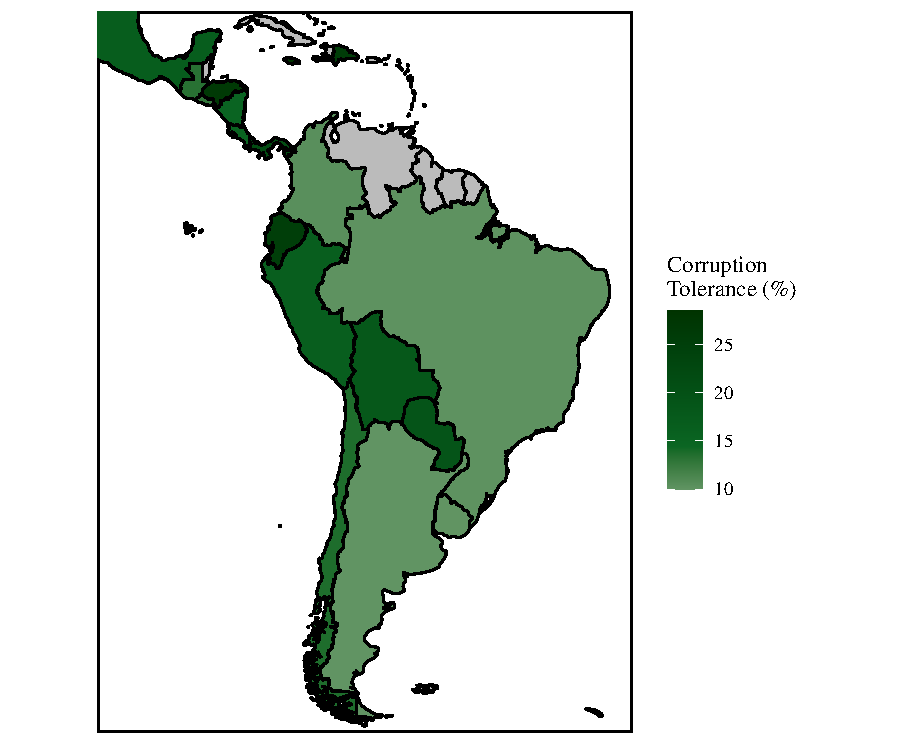
\includegraphics{images/ctol_map.pdf}
    \end{center}

A choropleth map showing corruption tolerance percentages across Latin America in 2019, where Ecuador places third in the most corruption tolerant countries. Darker areas imply higher percentages of corruption tolerance. Figure prepared by the author with data from the \textregistered AmericasBarometer 2018/19. 
\end{figure}

This paper aims to investigate the determinants of the largest corruption tolerance increase in Ecuador, seen from 2014 to 2016, as it can be seen in Figure \ref{fig:ctoly}. This period coincided with two key events in the country. First, the popularity of the governing regime sharply dropped for the first time in a decade \parencite{Quillupangui.2016}. Second, the country faced an economic recession \parencite{Weisbrot.2017}. The present paper will seek to relate  This is done by estimating a binary-outcome model through logistic regression, which relates the probability of tolerating corruption to several individual-level public opinion and economic indicators using the data from the AB. It is determined that changes in presidential job approval as well as in political wing preferences during the 2014 and 2016 period could have influenced the corruption tolerance increase. It is also found that those not unemployed justified corruption more in 2016 relative to those who were unemployed.

% Corruption Tolerance Time Series Graph

\begin{figure}[htbp]
\label{fig:ctoly}
\caption{Percent of Ecuadorians who justify corruption, by year}
\begin{knitrout}
\definecolor{shadecolor}{rgb}{0.969, 0.969, 0.969}\color{fgcolor}

{\centering 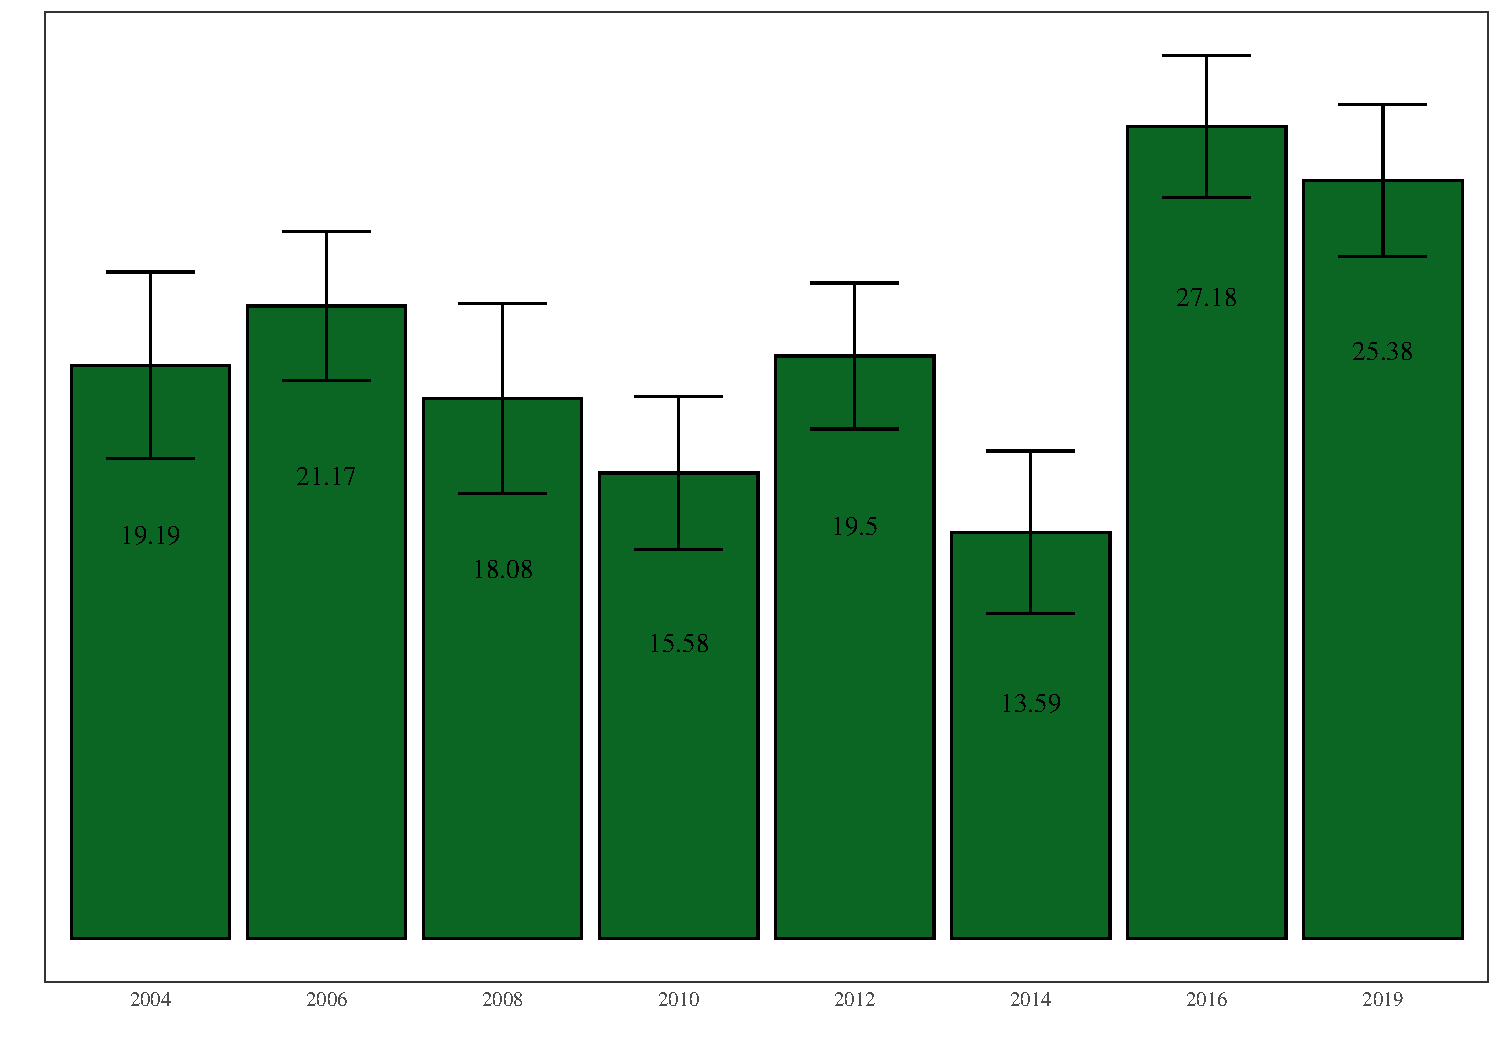
\includegraphics[width=\maxwidth]{figure/ctol_graph-1} 

}


\end{knitrout}


The evolution of corruption tolerance for Ecuador. The largest increase is seen from 2014 to 2016. Error bars show 95\% confidence intervals, considering survey design effects. Figure prepared by the author, with the open-access AB data.
\end{figure}

Changes to the attitudes toward corruption can be important for studying corruption incidence. A higher degree of corruption tolerance will eventually lead to larger corruption environments \parencite{Campbell.2014}. Learning what drives corruption tolerance can then foster better policymaking and citizen attitudes which steers individuals away from becoming involved in corruption.

The rest of the paper proceeds as follows. The following section gives an institutional and historical background of the paper's setting, Ecuador. Section 3 reviews the relevant literature. Section 4 develops the empirical methodology. Section 5 reviews the results from the empirical estimation. Section 6 discusses these results, and Section 7 concludes. 

\section{Institutional and Historical Context}





% Institutional Background Child Document



% Context .Rnw File


\section{Institutional and Historical Background}

\end{document}
